\documentclass[10pt]{article}
\usepackage{tikz}
\usetikzlibrary{shapes.misc}
\usepackage[margin=0cm]{geometry}
\pagestyle{empty}
\tikzstyle{every node}=[cross out, draw, red]

\begin{document}

\vspace*{\fill}
\begin{center}
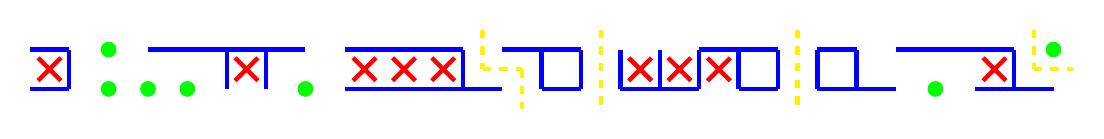
\begin{tikzpicture}[x=0.5cm, y=-0.5cm, ultra thick, blue]
% Walls
    \draw (0,0) -- (1,0);
    \draw (3,0) -- (7,0);
    \draw (8,0) -- (11,0);
    \draw (12,0) -- (14,0);
    \draw (17,0) -- (19,0);
    \draw (20,0) -- (21,0);
    \draw (22,0) -- (25,0);
    \draw (0,1) -- (1,1);
    \draw (8,1) -- (12,1);
    \draw (13,1) -- (14,1);
    \draw (15,1) -- (17,1);
    \draw (18,1) -- (19,1);
    \draw (20,1) -- (22,1);
    \draw (24,1) -- (26,1);
    \draw (1,0) -- (1,1);
    \draw (5,0) -- (5,1);
    \draw (6,0) -- (6,1);
    \draw (11,0) -- (11,1);
    \draw (13,0) -- (13,1);
    \draw (14,0) -- (14,1);
    \draw (15,0) -- (15,1);
    \draw (16,0) -- (16,1);
    \draw (17,0) -- (17,1);
    \draw (18,0) -- (18,1);
    \draw (19,0) -- (19,1);
    \draw (20,0) -- (20,1);
    \draw (21,0) -- (21,1);
    \draw (25,0) -- (25,1);
% Pillars
    \fill[green] (2,0) circle(0.2);
    \fill[green] (26,0) circle(0.2);
    \fill[green] (2,1) circle(0.2);
    \fill[green] (3,1) circle(0.2);
    \fill[green] (4,1) circle(0.2);
    \fill[green] (7,1) circle(0.2);
    \fill[green] (23,1) circle(0.2);
% Inner points in accessible cul-de-sacs
    \node at (0.5,0.5) {};
    \node at (5.5,0.5) {};
    \node at (8.5,0.5) {};
    \node at (9.5,0.5) {};
    \node at (10.5,0.5) {};
    \node at (15.5,0.5) {};
    \node at (16.5,0.5) {};
    \node at (17.5,0.5) {};
    \node at (24.5,0.5) {};
% Entry-exit paths without intersections
    \draw[dashed, yellow] (11.5,0.5) -- (12.5,0.5);
    \draw[dashed, yellow] (25.5,0.5) -- (26.5,0.5);
    \draw[dashed, yellow] (11.5,-0.5) -- (11.5,0.5);
    \draw[dashed, yellow] (12.5,0.5) -- (12.5,1.5);
    \draw[dashed, yellow] (14.5,-0.5) -- (14.5,1.5);
    \draw[dashed, yellow] (19.5,-0.5) -- (19.5,1.5);
    \draw[dashed, yellow] (25.5,-0.5) -- (25.5,0.5);
\end{tikzpicture}
\end{center}
\vspace*{\fill}

\end{document}
